\title{Syllabus for A History of Science in Latin America: INTD290}
\author{Dr. Jordan Hanson - Whittier College Dept. of Physics and Astronomy}
\date{\today}
\documentclass[10pt]{article}
\usepackage[a4paper, total={18cm, 27cm}]{geometry}
\usepackage{outlines}
\usepackage{hyperref}
\usepackage{graphicx}
\begin{document}
\maketitle

\begin{abstract}
Scientific inquiry was a cultural practice of the Maya, Aztec, and Inca civilizations. Colonial Spanish and Portuguese introduced the scientific method to the continent, which local communities incorporated to form the tradition of Latin American science. In the 19th century, the push for national independence was connected to a drive for scientific progress.  In the 20th century, science and technology became as omnipresent in Latin America as in the United States and Europe. However, some still view Latin American scientific achievements as derivative or peripheral to Euro-American science.  This course will provide a historical overview of the history of science in Latin America from the 16th century to the present. We will engage with the science through detailed discussions of essays exploring natural history, medicine and public health, the eighteenth-century Enlightenment, and contemporary physics and astronomy research. Interactive activities will demonstrate how the Maya, Aztec, and Inca performed calculations and made measurements, and compare the results those of other cultures. Students will engage in self-designed projects to replicate experiments done by ancient or Enlightenment-era Latin American scientists. Finally, we will cover how cutting-edge physics and astronomy research is being performed right now in Latin America.
\end{abstract}
\noindent
\textit{\textbf{Pre-requisites}: None} \\
\textit{\textbf{Course credits, Liberal Arts Categorization}: 3 Credits, CON2/CUL4} \\
\textit{\textbf{Regular course hours and location}: Monday through Friday, 8:00-9:15.  Synchronous time corresponds to meeting together via Zoom or in person, asynchronous time corresponds to engaging with pre-recorded content and thinking through content that prepares you for the homework and reading quizzes.} \\
\textit{\textbf{Instructor contact information}: 
\begin{enumerate}
\item Email: jhanson2@whittier.edu
\item Cell: 562.351.0047
\item Zoom ID / pass: 796 092 0745 / 667725
\item YouTube Channel: \url{www.youtube.com/918particle}
\item Book online appointments: \url{https://fgucmvjkylvmgqfsco.10to8.com}
\end{enumerate}}
\textit{\textbf{Office hours}: Please use the booking service to schedule Zoom meetings: \url{10to8.com} as above.} \\
\textit{\textbf{Attendance/Absence}: Students are required to log in for the morning Zoom sessions, however the asynchronous content may be digested on the students' individual schedules}.\\ 
\textit{\textbf{Late work policy}: Late work is generally not accepted, but is left to the discretion of the instructor.} \\
\textit{\textbf{Text}: ``Science in Latin America: A History,'' edited by Juan Jos\'{e} Salda\~{n}a.  (University of Texas Press, 2010).  Note that this book can be purchased as an e-Book via the Kindle App, and the Kindle App is free.} \\
\textit{\textbf{Grading}: There will be one take-home midterm, one (optional) final exam, and weekly reading quizzes.  There will also be homework assignments based on the text and independent research, submitted via Moodle.  Finally, there will be a self-designed project and presentation given at the end of the term.  Grading percentages are shown in Tab. \ref{tab:grades}.  Note that the final exam will be optional. The final project is a good opportunity for the use of Digital Storytelling.  For more information, see \url{https://diglibarts.whittier.edu} and contact Sonia Chaidez: \url{schaidez@whittier.edu}. } \\

\begin{table}[h]
\centering
\begin{tabular}{| c | c |}
\hline
Item & Percentage \\ \hline \hline
Reading quizzes & 20 \% \\ \hline
Homework assignments & 20 \% \\ \hline
Midterm & 20 \% \\ \hline
Final & 20 \% \\ \hline
Final Project + Presentation & 20\% \\ \hline
\end{tabular}
\begin{tabular}{| c | c |}
\hline
Item & Percentage \\ \hline \hline
Reading quizzes & 25 \% \\ \hline
Homework assignments & 25 \% \\ \hline
Midterm & 25 \% \\ \hline
Final Project + Presentation & 25\% \\ \hline
\end{tabular}
\caption{\label{tab:grades} (Left) These are the grade settings with the final exam included. (Right) These are the grade settings without the final exam.  The final exam is optional.}
\end{table}
\vspace{0.5cm}
\textit{\textbf{Grade Settings}: $\geq 60\%, <70\%$ = D, $\geq 70\%, <80\%$ = C, $\geq 80\%, <90\%$ = B, $\geq 90\%, <100\%$ = A.  \\ Pluses and minuses: 0-3\% minus, 3\%-6\% straight, 6\%-10\% plus (e.g. 79\% = C+, 91\% = A-)} \\ \\
\textit{\textbf{ADA Statement on Disability Services}: The Americans with Disabilities Act (ADA) is a federal anti-discrimination statute that provides comprehensive civil rights protection for persons with disabilities. Among other things, this legislation requires that all students with disabilities be guaranteed a learning environment that provides for reasonable accommodation of their disabilities. If you believe you have a disability requiring an accommodation, please contact Disability Services: disabilityservices@whittier.edu, tel. 562.907.4825.} \\
\textit{\textbf{Academic Honesty Policy}: \url{http://www.whittier.edu/academics/academichonesty}}

\textit{\textbf{Policy due to COVID-19}: Our course combines in-person discussions and activities with online Zoom meetings and asynchronous pre-recorded content.
\begin{enumerate}
\item Class will meet via Zoom usually three days per week.  There will be asynchronous activities distributed through Moodle that do not require us to meet over Zoom.
\item Group project results will be presented via Zoom during the last week of class.
\item \textbf{Students may opt-out of taking the final exam.}  In order to accommodate students' preparation for the Fall semester, the final exam is optional.  If one does not take it, the assignment weights for the final grade will be those given in Tab. \ref{tab:grades} (right).
\item The final project can be created in one of two options.  Option A: 3000-4000 word essay that includes maps, figures, and diagrams.  Option B: Digital liberal arts style, in the form of video or digital book form that educates the class on a topic.  Regardless of the option, students will all present their work to the class at the end of the module.
\end{enumerate}}

\textit{\textbf{Course Objectives}:}
\begin{itemize}
\item To practice written and oral expression of technical ideas.
\item To practice, in particular, the style of writing specific to science and the history of science
\item To develop an appreciation for the growth and evolution of scientific processes in Latin American culture over the last several centuries
\item To broaden our perspective regarding the practice of science in Latin America over the last several centuries
\item To understand in detail several major Latin American scientific efforts and their relevance to the broder scientific community
\item \textit{Note: for the most part, the \textbf{actors} in this history are called Creole by the authors of the text.  These are individuals of both Latin and Indigenous descent who spoke Spanish or Portugese, and performed academic, scientific, and development activities on behalf of their native Latin American country.  One central thesis of the course is that Creole elites and clergy are largely responsible for initiating modern science in Latin America.}
\end{itemize}

\textit{\textbf{Course Outline}:}
\begin{outline}[enumerate]
\1 \textbf{Unit 0}: Examples of pre-Columbian scientific processes in Latin America
\2 General outline of course, terminology from philosophy, Catholic terminology, geographic terminology, scientific notation, Nahuatl vocabulary, Spanish vocabulary
\2 Reading and discussion: The herbal medicine and comparative medicine of the 16th and 17th century
\3 Comparisons of treatments
\3 The theory of the four humours: medieval medicine carried from Europe to Latin America
\3 Indigenous treatments carried from Latin America to Europe
\3 Production of medicines on a mass scale
\2 Activities: Methods of computation and measurements of time in pre-Columbian Latin America
\3 The Quipu (Incan Empire), base 10 number systems, data representation
\3 The Maya number system, calendars and astronomical calculations
\3 Kepler's Laws, and deducing the structure of the solar system
\2 Reading quiz: Chapter 1 of the text
\2 Connection to Physics: skip to next week
\1 \textbf{Unit 1}: The Enlightenment in the Spanish Empire, part I: Nueva Espa\~{n}a (Mexico)
\2 Reading and discussion: Development of Enlightenment thought in Nueva Espa\~{n}a with a focus on Mexico
\3 The four viceroyalties (\textit{virreinatos}) of the Spanish colonies: agriculture and mining as an invitation to do science
\3 The spread of knowledge throughout Latin America, and the creation and cultivation of knowledge, private libraries, scientific societies and literary magazines
\3 The Catholic Church, The Society of Jesus (Jesuits), the Dominican Order of Preachers (OP), and Scholasticism
\3 Galileo, Kepler, the heliocentric universe, and the Inquisition
\3 Sir Isaac Newton and the advent of the scientific method
\2 Activities: Illustrations of the time period
\3 Timelines of discoveries: Galileo, Kepler and Brache, Newton, The American and French Revolutions
\3 Geographical illustrations: the four virreinatos, capital cities, nascent universities
\3 Cosmic rays, the solar wind, and magnetic fields
\3 The 4 categories of Mexican adoption of The Enlightenment
\2 Reading quiz: Chapter 2 of the text
\2 Connection to Physics: cosmic rays, the 1789 solar event and the aurora, Milagro, HAWC
\1 \textbf{Unit 2}: The Enlightenment in the Spanish Empire, part II: Nueva Granada and Peru (Columbia, Venezuela, Panama, Ecuador, Peru)
\2 Reading and discussion: The Jesuits, Dominicans, Scholasticism and the New Physics
\3 What constitutes a university?  From whom is the authority to teach derived?  What is a degree and who receives and gives them?
\3 Santa Fe de Bogot\'{a}, Quito, y Caracas
\3 Holy Scripture and the system of the world: the basic diagram
\3 Newtonian physics and the scientific method, the philosophy of Ren\'{e} Descartes, and new systems of the world from Copernicus, Kepler and Brache
\3 The explusion of the Jesuits from the Spanish Empire, and Dominican educational influence
\3 Geodetic expeditions, La Expedici\'{o}n Bot\'{a}nica
\2 Activities: Geographical calculations
\3 Latitude and longitude
\3 Triangulation and distance
\3 Kepler's Laws
\2 Connection to Physics: The optical obervatories of the Andes mountain range
\1 \textbf{Midterm exam:} Take-home exam at the end of Week 4
\1 \textbf{Unit 3}: Latin American expeditions, European and Latin American discovery
\2 Brief remarks about \textit{History and Current Status of Modern Science in Antarctica}, and the tradition of exploration literature
\2 Reading and discussion: Examples of collaboration in Latin America: the Church, the Viceroyal, and the Home Country
\3 The European expeditionary tradition and the realization that the exploration of the planet would soon be complete
\4 Example of Captain Cook, the 1769 transit of Venus, the astronomical unit
\4 Antarctic exploration and the competition between Robert Falcon Scott and Roald Amundsen
\3 Latin American expeditionary tradition
\4 Jesuit examples and the great chain of being, moral and natural histories, notions of equality
\4 Cartography of the interior of Latin America
\4 Flora and fauna, Linneaen classification
\4 Medicinal and economic opportunity
\2 Activities: Cartography
\3 Understanding vectors
\3 Trigonometry, vectors, directional headings
\3 Calculating distances in the interior of Latin America
\2 Reading quiz: Chapter 4 of the text
\2 Connection to Physics: The story of the Pierre Auger Observatory, and ultra-high energy cosmic rays
\1 \textbf{Unit 4}: Modern Science and Nationalism in Latin America during the 1800s
\2 Reading and discussion: Independence from Spain
\3 Why did the Creole elites decide to break away from Spain?
\3 Modernization and the scientific basis for the new system
\3 Economic, educational, and medical reforms
\2 Expeditions near the southern tip of Latin America and an essay by Barry Lopez
\3 \textit{Note: Barry Lopez was a fantastic author from Los Angeles who passed away this Christmas Day, 2020.  May he rest in peace, and thank you for your interesting and wondrous writing.}
\2 Reading Quiz: Selected passages from Chapter 5 of the text.
\1 \textbf{Unit 5 and final week of course}: Medicine, Public health in Latin America, 19th century - present
\2 Reading quiz: Selected passages from Chapters 6 and 8 of the text
\2 \textit{No additional assignments, except to prepare for the final project presentation.}
\2 Connection to Medicine: Modern excellence in biomedical research in Latin America
\2 \textit{Final project presentations}
\3 Option A: 3000-4000 word essay that includes maps, figures, and diagrams. The paper will be shared with the professor via Google Docs, and presented to the class via Zoom.
\3 Option B: Digital liberal arts style, in the form of video or digital book form that educates the class on a topic.  The project will be shared with the professor via Google Docs, and played or demonstrated for the class via Zoom.
\end{outline}
\begin{figure}[hb]
\centering
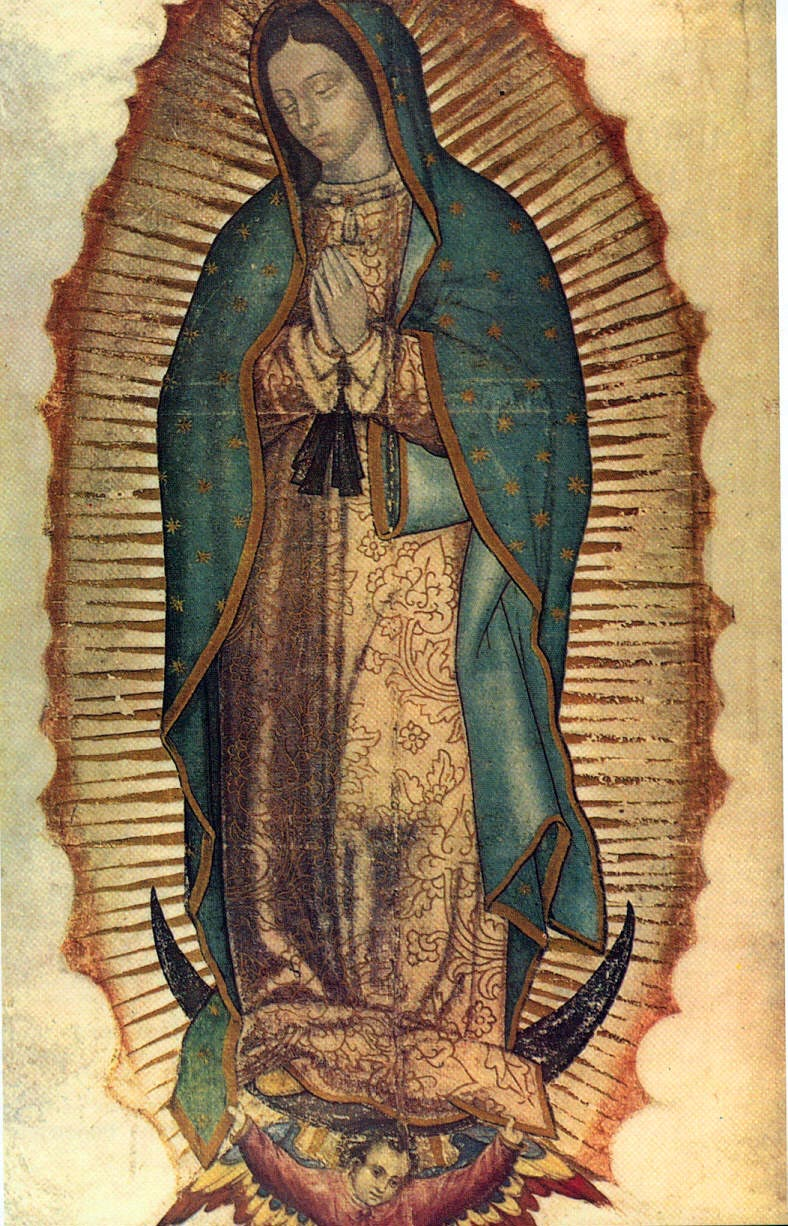
\includegraphics[width=8cm]{virgen.jpg}
\caption{\textit{The sacred image of the Virgin of Guadalupe, from December 1531.  Currently resides in the Shrine of Our Lady of Guadalupe in Mexico City.}  In addition to becoming a religious icon, this symbol has also been a focus of scientific study and a symbol of transition between the past and the modern era in Mexico.}
\end{figure}
\end{document}
